% Very simple template for lab reports. Most common packages are already included.
\documentclass[a4paper, 11pt]{article}
\usepackage[utf8]{inputenc} % Change according your file encoding
\usepackage{graphicx}
\usepackage{url}
\usepackage{parskip}
\usepackage{float}


%opening
\title{Report 2: Discovery of Frequent Itemsets and Association Rules }
\author{Laila Niazy, Svenja Raether}
\date{\today{}}

\begin{document}

\maketitle

\section{Introduction}

The objective of assignment two is to implement the Apriori algorithm for finding frequent itemsets with support of least s using the given dataset of sales transactions. Further, we needed to develop and implement an algorithm for generating association rules between the discovered frequent itemsets from the previous step. The rules must have support of least s and confidence of least c, where s and c are given as input parameters.

\section{Description of the solution}

In this section, we will describe our implementation, which is divided into two main parts: finding frequent items and their corresponding association rules. \newline

However, before we go through each function, we will give an overview of our git repository structure.
We have two folder in the first level and two python-files. The folder "Dataset" contains the given dataset of sales transactions and the folder "Report" contains the report. The file, which is called \textit{rules.py}, contains all the functions used to extracted the association rules from the frequent itemsets. The other file, which is called \textit{apriori.py}, is the main-executable file and contains the functions needed to extract the frequent items and imports the \textit{rules.py} to output the association rules as well.

\subsection{Finding Frequent Items}
In this subsection, we will go through each function found in \textit{apriori.py}.

\paragraph{\textit{getSupport.py}}
This function takes as an input a dict with the itemset as key and the count of how many times appeared as value and an integer with the number of transaction in our dataset.
The count of each itemset is divided by the number of transaction and give us the support. Using an if-function, we check if the calculated supported is larger or equal the s, which is the min-support value. If this statement is true, the support value is put in a dict, called items to its corresponding key, which is the itemset. This means we get as an output a dict with the following shape: {itemset:support}.

\paragraph{\textit{flatten\_tuples.py}}
This function takes tuples as input and flattens them into a set, which is given as an output. We use the data structure "set()" to make sure none of the tuple entries are repeated.

\paragraph{\textit{generateCandidates.py}}
This function takes the four following inputs: the dataset path, the number of frequent items from the previous step, \textbf{s} and the count, which tells us how many items are in a set of the frequent itemset, e.g. singletons have the count 1. In the beginning, we initialize 3 values. First, a frequent itemset with the datastructure set() called final\_candidates. Second, a default dictionary, which contains the possible candidates as keys and how many times they appear in the transaction as value and finally the number of transactions, which is an integer. \newline

Using the count, we differentiate between extracting singletons, doubletons and the rest k-candidates. In each if-function, we iterate through each transaction line in the dataset and increment the number of transaction after every line. To extract the singletons, we split each transaction line into items and iterate over the items. Using the default dict, we save each item as a key and increment the value by one each time the key/item is found in another transaction line. After we have looped over all transaction lines and their items, we input the default dict with the possible candidates and their count into \textit{getSupport.py} to get the dict with the itemset and their support and this is given as the final output. \newline

To create the doubletons, we use the singletons calculated in the first step, which are give as the keys of the dictionary and convert them into a set to get ride of any reappearing values. We again loop over the transaction lines and get the intersection of each transaction line the singletons-set we have. The items, that intersect, are combine into multiple tuples. Next, we take the multiple tuples and iterate through one by one and save each tuple as a key and increment the value by one each time the tuple is found in another transaction line. Again here, the default dict with the possible candidates and their count into \textit{getSupport.py} to get the dict with the itemset and their support and this is given as the final output. \newline

The same process is repeating when we have more than two items in a set. However, the k-frequent-candidates we get from the previous step, are k-tuples, which are flattened into a set and then combined into k+1-tuples.




\paragraph{\textit{findFrequentItems.py}}
This function takes as input the path of our dataset and the min-support value \textbf{s} and gives as output a dict with count being the key and the dict, that we get from \textit{generateCandidates.py} containing all frequent items that are larger than \textbf{s} and their support, being the value. Count is the number of items in the sets we find frequent and is incremented after every loop. In this function, we have a while loop, which is always true until the if-condition, which checks if the list() returned by \textit{generateCandidates.py}-function is empty, is fulfilled. 

\subsection{Finding Association Rules}
This part solves the second sub-problem. It covers an algorithm to generate association rules between frequent itemsets discovered by using the Apriori algorithm in a dataset of sales transactions. 
The implemented algorithm is based on the chapter 5.3 Rules Generation of the book Introduction to Data Mining (2nd edition) [1]. 


\paragraph{\textit{generateRules.py}}
This function is used to call the rule generation. It takes the itemset of frequent items with a support of s (which is the result of the first part) and the minconfidence (confidence at least c). 
The function iterates over the input dictionary and generates a ruleset for each entry in the dictionary with the frequent items. It skips the entries where the key equals 1 because association rules cannot be generated out of only singletons. 

It iterates over each given frequent itemset. It takes another copy of the itemset for all possible consequents of itemsize m=1. Then it calculates the confidence according to the definition and compares it with the minconf. If the confidence is larger or equal to the minconf the rule will be saved and the items of the right side of the rule stored in a list. This list will be used to generate the consequents (right side) of size m+1. If there are no consequents for m+1 it continues with the next item.
This way, we avoid the testing and generation of rules which can be excluded (based in the knowledge of low confidence of the preceding test). The pruning is illustrated in Figure 1. 



\begin{figure}[H]
  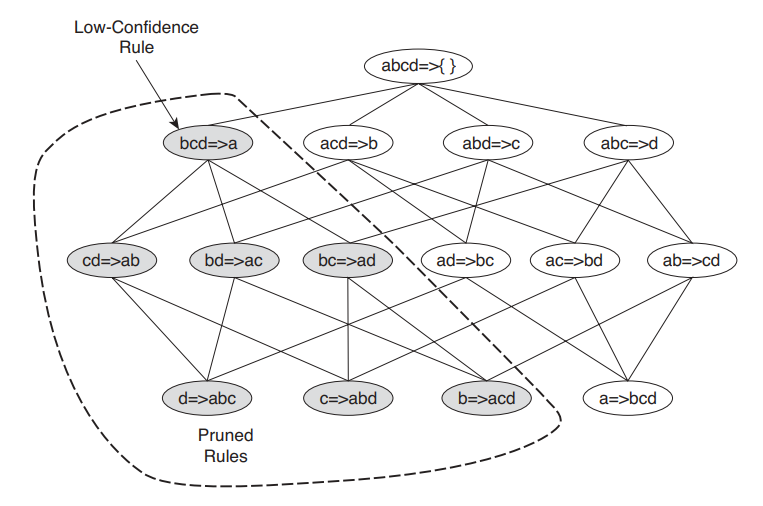
\includegraphics[width=\linewidth]{res/rules.PNG}
  \caption{Pruning of association rules using the confidence measure (Taken from source [1])}
  \label{fig:rules}
\end{figure}



\section{Evaluation and Results}

\paragraph{Testing with s (min-support value)}
In this test, we vary the value \textbf{s} and depending on that we either get more frequent items or less. The lower \textbf{s} is the more frequent items we get and vice versa. The results can be observed in Tab.\ref{tab:results_s}.
\begin{table}[H]
	\centering
	\begin{tabular}{|c|c|}
		\hline
		min-support  s & Number of frequent itemsets \\\hline
		$s=0.003$ & 4552\\
		$s=0.005$ & 1073 \\
		$s=0.01$ & 385  \\
		$s=0.02$ & 155 \\
		\hline
	\end{tabular}
	\caption{Number of frequent itemsets with changing s}
	\label{tab:results_s}
\end{table}
\paragraph{Testing with c (min-confidence value)}

The test results of the rule generation are shown in the table below. It shows the number of rules generated for a given support (0.003, 0.005, 0.01, and 0.02) and confident thresholds (0.6, 0.75, and  0.9).

\begin{table}[H]
	\centering
	\begin{tabular}{|l|c|c|c|c|c|} 
		\hline
		support/confidence &$s = 0.003$ &  $s = 0.005$ & $s = 0.01$ & $s = 0.02$  \\\hline
		$s=0.6$ &19877   &1072       &5& - \\
		$s=0.75$ &18494   &964       &3& -\\
		$s=0.9$ &11856    &532       &2&-\\
		\hline
	\end{tabular}
	\caption{Results of the number of association rules based on given support and confidence}
	\label{tab:results_h_2}
\end{table}

The results show: the higher the support is the less frequent items are found by the apriori generation. This influences the number rules. We generate less rules the higher the support threshold is. Furthermore, an increase in the confidence threshold also reduces the number of rules found in the input set since we filter out a larger amount of rules. The last column (support = 0.02) produces only singletons as frequent items. Therefore, no rules can be generated.

\paragraph{Testing with time}
In this test, we again vary the value \textbf{s} and depending on that we observe how long the computation for extracting the frequent items and association rules takes. The lower \textbf{s} is the more frequent items we get and thus the longer our computation takes. The results can be observed in Tab.\ref{tab:results_t}.
\begin{table}[H]
	\centering
	\begin{tabular}{|c|c|c|}
		\hline
		min-support  s & time for frequent itemset & time for association rules\\\hline
		$s=0.003$ & 59.9 & 0.06\\
		$s=0.005$ & 6.60 & 0.005 \\
		$s=0.01$ & 2.34 &  0.00008 \\
		$s=0.02$ & 0.99  &  0.000007\\
		\hline
	\end{tabular}
	\caption{Computation time results with varying s and c = 0.9}
	\label{tab:results_t}
\end{table}


\section{Instructions}
Here we will go through the instructions on how to run our implemented function.The only file needed to be run is the \textit{apriori.py} using the following command: 

\textbf{python apriori.py}


The default value for $s$ is 0.01, if the user wants to change it, they can enter it after this statement: 

\textbf{Enter min-support value, which should be between 0 and 1:} 

If the statement is left blank by clicking enter, the default value will be used.

Furthermore, the default value for c is 0.9 and can also be change by the user, by entering it after the statement: 

\textbf{Enter a min-confidence value, which should be between 0 and 1:} 

If again left blank, the default value be used here.

\begin{table}[H]
		\centering
		\begin{tabular}{|l|c|c|c|c|} 
			\hline
			$\delta$ & Edge-Cuts &  Swaps & Migration & $T_{min}$ \\\hline
			 0.1 & 1003 & 579353 & 3537 & 0.001\\
			0.3 &  1082 & 621609 & 3532 & 0.001\\
			0.5 & 893 & 568771 & 3525 & 0.001 \\
			0.8 & 964 & 593501 & 3550 & 0.001 \\
			 0.85 & 907 & 577028 & 3560 & 0.001 \\
			0.90 & 1036 & 573972 &  3550 & 0.001 \\
			 0.95 & 1117 & 60653 & 3528 & 0.001 \\
			0.99 & 1026 & 603009 &  3534 & 0.001 \\
			 0.1 & 904 & 577316 & 3540 & 0.00001\\
			0.3 & 964 & 585100 &3565 & 0.00001 \\
			 0.5 & 978 & 577157 & 3560 & 0.00001\\
			 0.8 & 1070 & 611676 & 3560 & 0.00001\\
			 0.85 & 906 & 597366 & 3552 & 0.00001\\
			0.90 &  1016 & 578522 & 3554 & 0.00001\\
			0.95 & 1025 & 583228 & 3545 & 0.00001\\ 
			0.99 & 1011 & 587892 & 3559 & 0.00001\\
			 0.1 & 1038 & 593295 & 3533 & 0.0000001\\
			0.3 & 1050 & 588085 & 3504 & 0.0000001\\
			0.5 & 1052 & 603505 & 3513 & 0.0000001\\
			 0.8 & 1146 & 608373 & 3531 & 0.0000001\\
			 0.85 & 1259 & 622790 & 3554 & 0.0000001\\
			 0.90 & 978 & 597213 & 3541 & 0.0000001\\
			0.95 & 1164 & 638684 & 3519 & 0.0000001\\
			\textbf{0.99} & \textbf{876} & 588544 & 3516 & \textbf{0.0000001}\\
			
			\hline
		\end{tabular}
		\caption{Tuning $\delta$ and $T_{min}$ for the graph \textit{3elt} with hybrid sampling, $\alpha=2$ \& SA}
		\label{tab:3elt_delta_1}
	\end{table}
	\begin{table}
		\centering
		\begin{tabular}{|l|c|c|c|c|} 
			\hline
			$\delta$ & Edge-Cuts &  Swaps & Migration  & $T_{min}$  \\\hline
		 0.1 &  2056 & 1172330 & 1779 & 0.001\\
		0.3 & 2074 & 1173278 & 1831 & 0.001\\
		 0.5 & 2029 & 1165578 & 1799 & 0.001\\
		0.8 & 2048 & 1165380 & 1770 & 0.001\\
		0.85 & 2032 & 1158499 & 1759 & 0.001\\
		0.90 & 2438 & 1344630 & 1786 & 0.001\\
		0.95 & 2053 & 1162821 & 1767 & 0.001\\
		 0.99 & 2123 & 1202484 & 1783 & 0.001\\
		 0.1 & 2055 & 1169224, & 1783 & 0.00001\\
		  0.3 & 2027 & 1159600 & 1793 & 0.00001\\
		  0.5 & 2034 & 1153010 & 1789 & 0.00001\\
		  0.8 & 2143 & 1203337 & 1824 & 0.00001\\
		  0.85 & 2110 & 1199560 & 1775 & 0.00001\\
		 0.90 &  2032 & 1151197 & 1802 & 0.00001\\
		 \textbf{0.95} & \textbf{2019} &1148646 & 1769 & 0.00001\\
		 0.99  & 2101 & 1204757 & 1813& 0.00001\\
		 0.1 & 2069 & 1183907 & 1823 & 0.0000001\\
		 0.3  & 2087 & 1196444 & 1805 & 0.0000001\\
		 0.5  & 2033 & 1160702 & 1782 & 0.0000001\\
		 0.8 & 2130 & 1199781 & 1804 & 0.0000001\\
		 0.85 & 2080 & 1181129 & 1801 & 0.0000001\\
		 0.90 &  2038 & 1166066 & 1809 & 0.0000001\\
		  0.95 & 2085 & 1174323 & 1799 & 0.0000001\\
		 0.99 & 2035 & 1165881 & 1789 & 0.0000001\\
			\hline
		\end{tabular}
		\caption{Tuning $\delta$ and $T_{min}$ for the graph \textit{add20} with hybrid sampling, $\alpha=2$ \& SA}
		\label{tab:add20_delta_2}
\end{table}

\begin{table}[H]
	\parbox{.4\linewidth}{
		\centering
		\begin{tabular}{|l|c|c|c|} 
			\hline
			$\alpha$ & Edge-Cuts &  Swaps & Migration  \\\hline
			1.0  & 1783 & 1448283 & 3556 \\
			1.5 & 1089 & 657638 & 3524 \\
			\textbf{2.0} & \textbf{876} & 588544 & 3516\\
			 2.5 & 1046 & 587442 & 3548 \\
			 3.0 & 992 & 619293 & 3524'\\
			\hline
		\end{tabular}
		\caption{Tuning $\alpha$ for the graph \textit{3elt} with hybrid sampling, $\delta=0.98$, $T_{min} = 0.0000001$ \& SA}
		\label{tab:3elt_alpha}}
	\hfill
	\parbox{.4\linewidth}{
		\centering
		\begin{tabular}{|l|c|c|c|} 
			\hline
			$\alpha$ & Edge-Cuts &  Swaps & Migration  \\\hline
			1.0  & 2234 & 1358690 & 1799 \\
			 1.5 & 2053 & 1159501 & 1808 \\
			 \textbf{2.0} & \textbf{2019} & 1148646 & 1769 \\
			 2.5 & 2233 & 1262270 & 1795 \\
			 3.0 & 2265 & 1209053 & 1779 \\
			\hline
		\end{tabular}
		\caption{Tuning $\alpha$ for the graph \textit{add20} with hybrid sampling, $\delta=0.95$, $T_{min} = 0.00001$ \& SA}
		\label{tab:add20_alpha}}
\end{table}



\begin{table}[H]
	\centering
	\parbox{.35\linewidth}{
		\begin{tabular}{|l|c|c|c|} 
			\hline
			NSP & Edge-Cuts &  Swaps & Migration  \\\hline
			Hybrid & 876 & 588544 & 3516\\
			Random & \textbf{815} & 13121 & 3478\\
			Local &  4055 & 1613228& 3545 \\
			\hline
		\end{tabular}
		\caption{Comparing node selections policies with the optimal parameters: $\alpha=2$, $\delta=0.99$, $T_{min}=0.0000001$ \& SA}
		\label{tab:3elt_nodepolicy}}
	\hfill
	\parbox{.35\linewidth}{
		\centering
		\begin{tabular}{|l|c|c|c|} 
			\hline
			NSP & Edge-Cuts &  Swaps & Migration  \\\hline
			Hybrid & 2019 & 1148646 & 1769 \\
			Random & \textbf{1682} & 11126 & 1799	\\	
			Local & 3642 & 1690725 & 1447\\
			\hline
		\end{tabular}
		\caption{Comparing node selections policies with the optimal parameters: $\alpha=2$, $\delta=0.95$, $T_{min}=0.00001$ \& SA}
		\label{tab:add20_nodepolicy}}
	
\end{table}


\section{Sources}
[1] https://www-users.cs.umn.edu/~kumar001/dmbook/index.php, Chapter 5, p.26

\end{document}